\documentclass[11pt,letterpaper]{article}
\usepackage[margin=0.78in]{geometry}
\usepackage{mathptmx}
\usepackage[T1]{fontenc}
\usepackage[utf8]{inputenc}
\usepackage{amsmath,amssymb}
\usepackage{graphicx}
\usepackage{booktabs}
\usepackage{tabularx}
\usepackage{array}
\usepackage{xcolor}
\usepackage{xurl}
\usepackage{hyperref}
\usepackage{caption}
\usepackage[numbers,sort&compress]{natbib}
\usepackage{microtype}
\usepackage{ragged2e}

\hypersetup{
  colorlinks=true,
  linkcolor=blue!60!black,
  citecolor=blue!60!black,
  urlcolor=blue!60!black
}

\captionsetup{font=small,labelfont=bf}
\newcolumntype{L}[1]{>{\RaggedRight\arraybackslash}p{#1}}
\newcolumntype{C}[1]{>{\Centering\arraybackslash}p{#1}}
\newcolumntype{Y}{>{\RaggedRight\arraybackslash}X}
\setlength{\parskip}{0.38em}
\setlength{\parindent}{0pt}
\renewcommand{\topfraction}{0.90}
\renewcommand{\bottomfraction}{0.85}
\renewcommand{\textfraction}{0.08}
\renewcommand{\floatpagefraction}{0.75}
\sloppy

\title{\textbf{ClinVar Schema Stripping Drives Systematic Non-Qualifying Secondary Findings, Ancestry Disparities, and Opposite-Direction Lipid Calls Across Clinical Genome Pipelines}}

\author{
  Computational Clinical Genomics Audit Working Group$^{1}$\\
  \small $^{1}$Independent Open-Data Research Consortium (Correspondence: \texttt{reproducibility-archive@local})
}
\date{November 25, 2026}

\begin{document}
\maketitle

\begin{abstract}
\noindent
Clinical genome pipelines screen for actionable autosomal-dominant (AD) secondary findings (ACMG SF v3.3; 73 AD genes) using NCBI ClinVar pathogenic/likely pathogenic (P/LP) annotations. However, official ClinVar flat exports (\texttt{clinvar.vcf.gz}, \texttt{variant\_summary.txt.gz}, \texttt{submission\_summary.txt.gz}) omit \texttt{ModeOfInheritance}, collapse multi-submitter conditions into unstratified unions, and expose overlapping-gene \texttt{GENEINFO} bleed-through. Across all 7,427 gnomAD v4.1-observed AD P/LP alleles (4,799 high-callability 2--4$\star$), eight public pipelines---\texttt{Exomiser}, \texttt{AutoGVP}, \texttt{CPSR v2.4.0}, \texttt{SFtool}, \texttt{CPHI-DRAGEN-anno}, \texttt{viking-genes}, \texttt{OwnGenome}, and \texttt{DNA}---achieve 0.0--23.5\% specificity on non-qualifying alleles, yielding 5.3--6.6\% global carrier-weighted false discovery (12.8--13.9\% in South Asians; 2.0--2.5-fold SAS/NFE disparity). In 2,504 unrelated 1000 Genomes participants, 3/6 (50.0\%; 6.13/1,000) high-confidence South Asian AD calls are strictly recessive 3$\star$ \textit{RYR1} p.Arg3550Trp alleles, while \texttt{GENEINFO} bleed-through misassigns recessive \textit{NTHL1} p.Gln82Ter to \textit{TSC2} in 2/503 Europeans. In 411,351 UK Biobank exomes, all 13 misreturned 2--4$\star$ \textit{APOB} truncations lower Direct LDL-C ($\beta = -1.73$~SD, $p = 4.0\times 10^{-194}$), opposite to familial hypercholesterolemia controls ($+0.98$~SD \textit{APOB}; $+0.31$~SD \textit{LDLR}). SCV-XML inheritance and mechanism gating eliminates these errors at 100\% sensitivity on 3$\star$ AD curations, motivating upstream ClinVar \texttt{CLNMOI} emission.
\end{abstract}

\section{Introduction}
Opportunistic screening for secondary findings under ACMG SF v3.3 (84 genes: 73 autosomal dominant [AD], 8 autosomal recessive [AR], 3 X-linked) is now standard across clinical exome/genome services and population biobanks~\citep{lee2025acmgsf33,kerr2025viking}. Recent population audits have refined disease-specific allele-frequency thresholds~\citep{johnston2026daft} and quantified penetrance of predicted loss-of-function (pLoF) alleles in gnomAD v4~\citep{gudmundsson2025gnomad}, confirming that 2--4$\star$ ClinVar P/LP alleles rarely breach benign allele-frequency cutoffs. Yet literature searches across PubMed, Europe PMC, and OpenAlex through November 25, 2026 (search log archived in the reproducibility supplement) identified no prior multi-pipeline execution benchmark quantifying how widely deployed clinical and biobank pipelines handle \textit{allelic pleiotropy, dual mode of inheritance (MOI), opposite-direction molecular mechanisms, and overlapping-gene bleed-through} inside AD-listed ACMG SF genes.

Multiple AD-listed ACMG SF v3.3 genes harbor ClinVar P/LP alleles that do not meet ACMG SF v3.3 reporting criteria in simple heterozygotes: (i) \textit{RYR1}, listed for AD gain-of-function malignant hyperthermia susceptibility (MHS, \texttt{OMIM:145600})~\citep{johnston2021ryr1vcep}, also harbors abundant AR congenital myopathy missense and null alleles curated by the ClinGen Congenital Myopathies Variant Curation Expert Panel (VCEP)~\citep{snoeck2015ryr1}; (ii) \textit{TTN}, restricted by ACMG SF footnote~f to truncating variants in constitutively expressed cardiac exons (proportion spliced-in [PSI]~$>90\%$)~\citep{roberts2015ttn,lee2025acmgsf33}, contains non-truncating and low-PSI skeletal-myopathy alleles; (iii) \textit{APOB}, listed for AD familial hypercholesterolemia (FH, elevated LDL-C via defective receptor-binding missense alleles), contains pLoF alleles causing familial hypobetalipoproteinemia (FHBL, \texttt{OMIM:615558}), which \emph{lower} LDL-C and protect against coronary heart disease~\citep{peloso2019apob}; and (iv) \textit{CACNA1S} (AD MHS vs.\ AR congenital myopathy pLoF), \textit{DES} (dominant-negative AD vs.\ AR null alleles), \textit{LMNA} (cardiac vs.\ AR peripheral neuropathy), \textit{RET} (GoF MEN2 vs.\ LoF Hirschsprung disease), and \textit{VHL} (AD cancer vs.\ AR Chuvash erythrocytosis).

Direct inspection of official NCBI ClinVar GRCh38 distribution files (\texttt{2026-11-22})~\citep{landrum2025clinvar} exposes an ecosystem-wide upstream bottleneck that extends beyond VCF alone: \textbf{not only \texttt{clinvar.vcf.gz} (0/31 \texttt{\#\#INFO} tags), but also NCBI ClinVar's official tab-delimited \texttt{variant\_summary.txt.gz} and \texttt{submission\_summary.txt.gz} omit \texttt{ModeOfInheritance} completely.} Submission-level inheritance assertions survive solely inside multi-gigabyte ClinVar XML releases. Simultaneously, \texttt{CLNDN} and \texttt{CLNDISDB} collapse all submitters' disease strings into an unstratified union, allowing a legacy gene-level submission to attach AD OMIM identifiers to AR-only alleles, while \texttt{GENEINFO} lists every overlapping gene at a genomic locus. Here we combine (1) source-level and executable audits of eight pinned clinical, biobank, and open-source pipelines across the complete unbiased universe of 7,427 gnomAD-observed AD ACMG SF ClinVar P/LP alleles; (2) individual-level execution across all 2,504 unrelated (3,202 total) real 30$\times$ whole genomes from the 1000 Genomes Project~\citep{byrskabishop2022_1kg}; and (3) direct variant-level lipid and clinical outcome phenotyping across 411,351 UK Biobank exomes~\citep{backman2021ukbexome,zoodsma2025nmr,buniello2025opentargets}.

\section{Methods}
\subsection{Unbiased Complete-Universe Benchmark and ClinVar XML Reference Curation}
To avoid selection bias from small illustrative panels, our primary evaluation spans all 7,427 gnomAD v4.1-observed ClinVar P/LP alleles (non-conflicting Pathogenic or Likely pathogenic; 5,189 at 2--4$\star$; 4,799 at 2--4$\star$ with $\ge 80\%$ callability, $\text{AN}\ge 1{,}291{,}459$) across all 73 AD ACMG SF v3.3 genes, joined by exact GRCh38 \texttt{chr-pos-ref-alt} match to gnomAD v4.1 joint summary counts (807,162 individuals: 730,947 exomes and 76,215 genomes across NFE, AFR, AMR, EAS, and SAS)~\citep{chen2024gnomadv3,gnomadv41release2024}.

We established conservative reference labels distinguishing alleles meeting ACMG SF v3.3 reporting criteria (\texttt{MEETS\_ACMG\_SF}) from alleles not meeting criteria (\texttt{NOT\_MEETING}). First, we fetched live ClinVar VCV XML for all 117 3$\star$ Expert-Panel alleles across dual-mode and \texttt{lof=no} AD genes (including all 69 3$\star$ \textit{RYR1} alleles) plus all 28 2--4$\star$ pLoF alleles in non-\textit{RYR1}/\textit{APOB} \texttt{lof=no} genes. Ten 3$\star$ \textit{RYR1} alleles curated exclusively by the ClinGen Congenital Myopathies VCEP with explicit \texttt{ModeOfInheritance="Autosomal recessive inheritance"} were labeled non-meeting. Crucially, live XML audit identified genuine AD truncating variants inside putative \texttt{lof=no} genes---specifically 3$\star$ Cardiomyopathy VCEP \textit{TNNT2} p.Trp297Ter (last-exon NMD-escaping truncation) and 2$\star$ AD \textit{PLN} p.Leu39Ter (single-exon DCM allele, 31 gnomAD heterozygotes), as well as AD-annotated pLoFs in \textit{MYH7} and \textit{ACTA2}. We conservatively retained all 42 pLoF alleles across \textit{PLN}, \textit{MYH7}, \textit{MYH11}, \textit{ACTA2}, \textit{TNNT2}, \textit{TNNI3}, \textit{RYR2}, \textit{TMEM43}, and \textit{TNNC1} in \texttt{MEETS\_ACMG\_SF}, restricting non-meeting classification strictly to clinically established discordant mechanisms: \textit{RYR1} AR VCEP, pLoF, and non-MH alleles; \textit{APOB} FHBL pLoFs; \textit{TTN} non-truncating and low-PSI ($\le 90\%$ Cardiodb left-ventricular PSI) alleles; \textit{CACNA1S} and \textit{DES} AR-null pLoFs; \textit{LMNA} non-cardiac neuropathy alleles; and \textit{RET} LoF Hirschsprung alleles. This yields 665/7,427 all-star (179/4,799 high-callability 2--4$\star$) non-meeting alleles. We additionally evaluated our 24-variant heterozygous (\texttt{0/1}) executable panel (containing 15 discordant alleles, 1 high-PSI A-band \textit{TTN} p.Lys25729Ter verified via Cardiodb bounds, 4 AD positive controls, and 4 pure-AR heterozygous negative controls) as a targeted mechanism probe.

\subsection{Tiered Audit and Direct Execution of Eight Public Pipelines}
We shallow-cloned pinned releases of eight public workflows, separating clinical/biobank systems (\textbf{Tier A}) from open-source personal-WGS tools (\textbf{Tier B}):
\begin{itemize}\setlength{\itemsep}{1.5pt}
  \item \textbf{Tier A (Clinical \& Biobank):} (1) \texttt{Exomiser} (\texttt{98f4e0b}, Monarch Initiative / Genomics England~\citep{smedley2015exomiser}); (2) \texttt{AutoGVP} (\texttt{054e2b7}, CHOP / NIH Kids First~\citep{kim2024autogvp}); (3) \texttt{CPSR v2.4.0} (\texttt{7f68f9d}, Oslo University Hospital~\citep{nakken2021cpsr}); (4) \texttt{SFtool} (\texttt{0d72249}, Andalusian Health System); (5) \texttt{CPHI-DRAGEN-anno} (\texttt{974860d}, SickKids Toronto, analyst-triage candidate report); and (6) \texttt{viking-genes/clinvar\_pipeline} (\texttt{3ea7abe}, Univ.\ of Edinburgh~\citep{kerr2025viking}). We also audited \texttt{Talos v12.3.1} (\texttt{4aada15}, Australian Genomics~\citep{welland2026talos}) as a diagnostic MOI comparator.
  \item \textbf{Tier B (Open-Source WGS):} (7) \texttt{OwnGenome} (\texttt{c324b61}, compiled Rust binary \texttt{og}); and (8) \texttt{DNA} (\texttt{f459b22}).
\end{itemize}
Source-code rules were verified line-by-line across all eight repositories (\texttt{Exomiser} \texttt{ClinVarAlleleParser.java:116--140} and \texttt{ClinVarWhiteListReader.java:55--57}; \texttt{AutoGVP} \texttt{scripts/\allowbreak resolve-clinvar-intepretations.R:171--176, 257--278}), and unmodified executables for \texttt{CPSR v2.4.0}, \texttt{SFtool}, \texttt{CPHI-DRAGEN-anno}, \texttt{viking-genes}, \texttt{OwnGenome} (\texttt{og}), and \texttt{DNA} were executed directly on both the 24-variant GRCh38 VCF and real 1000 Genomes alleles.

\subsection{Individual-Level 1000 Genomes Real WGS Execution and gnomAD v4.1 Summary Bounds}
Because gnomAD provides aggregate variant-level \texttt{AC}/\texttt{AN}/\texttt{HOM} counts without joint individual genotypes, cross-variant sums cannot be treated as exact deduplicated counts of unique individuals. From per-variant heterozygous carrier rates $p_i = \max(0,\text{AC}_i - 2\cdot\text{HOM}_i)/(\text{AN}_i/2)$, we therefore report three explicit estimators across callability regimes ($\ge 80\%$ and $\ge 95\%$ of max autosomal $\text{AN}=1{,}614{,}324$): the cumulative carrier-instance rate $\sum_i p_i$ per 1,000 diploid sample-equivalents (Boole upper bound), the independence-model estimate $1-\prod_i(1-p_i)$, and the model-free single-variant Fr\'{e}chet lower bound $\max_i p_i$, accompanied by live gnomAD v4.1 GraphQL exome-vs.-genome callset verification.

To complement summary bounds with exact individual-level human genomes, we built a Tabix leaf-bin HTTP-range slicer over all 22 autosomes of the 1000 Genomes Project 30$\times$ NYGC GRCh38 phased WGS release (3,202 total individuals; canonical Phase~3 panel of 2,504 unrelated individuals across AFR [661], EAS [504], EUR [503], SAS [489], and AMR [347])~\citep{byrskabishop2022_1kg}. We extracted every individual carrier of any ClinVar P/LP allele across all 73 AD ACMG SF genes, verified live ClinVar XML SCV inheritance for all 26 observed alleles, and directly executed compiled Rust \texttt{OwnGenome} (\texttt{og}), R \texttt{CPSR v2.4.0}, and Python \texttt{SFtool} on those exact real-genome alleles.

\subsection{Direct Variant-Level Phenotyping in 411,351 UK Biobank Exomes}
To test whether misreturned \textit{APOB} truncating alleles produce opposite-direction biochemical phenotypes in measured human cohorts, we sliced the official EBI GWAS Catalog Tabix-indexed harmonized summary statistics of Backman et al.~\citep{backman2021ukbexome} (UK Biobank 454,787 exomes) across \textit{APOB} (\texttt{chr2:21001000--21045000}) and \textit{LDLR} (\texttt{chr19:11089000--11134000}) for three harmonized quantitative biomarkers on identical per-allele SD scales: Direct LDL-C (\texttt{GCST90079033}, UKB field 30780, $N=411{,}351$), Total Cholesterol (\texttt{GCST90079024}, field 30690, $N=412{,}075$), and Apolipoprotein~B (\texttt{GCST90079018}, field 30640, $N=410{,}113$). We computed inverse-variance weighted (IVW) group means, within-gene contrasts, and non-parametric Mann--Whitney $U$ tests across all matched 2--4$\star$ ClinVar P/LP alleles without exclusion, and queried Open Targets Platform~\citep{buniello2025opentargets} for UK Biobank clinical diagnoses, lipid-lowering medication use~\citep{backman2021ukbexome,karczewski2025panukb}, Nightingale NMR metabolomics ($N=434{,}646$)~\citep{zoodsma2025nmr}, and aortic stenosis ($N=2.85\text{M}$)~\citep{small2026as}.

\section{Results}
\subsection{Upstream Schema Stripping Affects Both Clinical Standards and Open-Source WGS Pipelines}
Source audit of \texttt{Exomiser} (\texttt{98f4e0b}) and \texttt{AutoGVP} (\texttt{054e2b7}) establishes that ClinVar inheritance loss is not confined to consumer tools. In \texttt{Exomiser}, \texttt{ClinVarAlleleParser.java:116--140} parses only \texttt{CLNSIG} and \texttt{CLNREVSTAT} while discarding \texttt{CLNDN} and \texttt{CLNDISDB} entirely, \texttt{ClinVarData.java:35--44} stores zero MOI attribute, and \texttt{ClinVarWhiteListReader.java:55--57} whitelists every undisputed 1--4$\star$ P/LP variant. In \texttt{AutoGVP}, \texttt{scripts/\allowbreak resolve-clinvar-intepretations.R:171--176} ingests NCBI's official \texttt{variant\_summary.txt.gz} and \texttt{submission\_summary.txt.gz}---confirming that neither tab-delimited ClinVar release carries \texttt{ModeOfInheritance}---and lines 257--278 bypass condition filtering on all non-conflicting P/LP alleles. Similarly, diagnostic MOI validator \texttt{Talos v12.3.1} (\texttt{validate\_moi.py:160--171})~\citep{welland2026talos} emits heterozygous ClinVar P/LP calls as \texttt{Autosomal Dominant} on \texttt{Monoallelic} gene panels without MOI ambiguity warnings.

\begin{table}[!t]
\centering
\caption{\textbf{Unbiased complete-universe benchmark across all 4,799 high-callability ($\ge 80\%$ AN) 2--4$\star$ ClinVar P/LP alleles in 73 AD ACMG SF v3.3 genes (4,620 meeting criteria; 179 non-meeting) across eight public pipelines.} Rates per 1,000 diploid sample-equivalents are Boole upper bounds from gnomAD v4.1 (independence-model estimates agree within $<0.11\%$; model-free SAS single-variant lower bound $=3.34/1{,}000$).}
\label{tab:unbiased}
\footnotesize
\setlength{\tabcolsep}{2.6pt}
\begin{tabularx}{\textwidth}{Y C{1.05cm} r r r r r r r r}
\toprule
\textbf{Pipeline (Pinned Commit)} & \textbf{Tier} & \textbf{FP / 179} & \textbf{Non-SF Spec.} & \textbf{Recall} & \textbf{Joint /1k} & \textbf{Joint FDR} & \textbf{NFE /1k} & \textbf{SAS /1k} & \textbf{SAS FDR (SAS/NFE)} \\
\midrule
\textbf{Exomiser} (\texttt{98f4e0b}) & A (Clin.) & 179 & 0.0\% & 100.0\% & 2.16 & 6.57\% & 2.12 & 4.28 & 13.27\% (2.02$\times$) \\
\textbf{AutoGVP} (\texttt{054e2b7}) & A (Clin.) & 179 & 0.0\% & 100.0\% & 2.16 & 6.57\% & 2.12 & 4.28 & 13.27\% (2.02$\times$) \\
\textbf{CPHI-DRAGEN}* (\texttt{974860d}) & A (Clin.) & 179 & 0.0\% & 100.0\% & 2.16 & 6.57\% & 2.12 & 4.28 & 13.27\% (2.02$\times$) \\
\textbf{Viking Genes} (\texttt{3ea7abe}) & A (Biob.) & 176 & 1.7\% & 97.9\% & 1.98 & 6.21\% & 1.95 & 4.28 & 13.87\% (2.20$\times$) \\
\textbf{CPSR v2.4.0} (\texttt{7f68f9d}) & A (Clin.) & 168 & 6.2\% & 100.0\% & 1.90 & 5.83\% & 1.79 & 4.24 & 13.16\% (2.36$\times$) \\
\textbf{SFtool} (\texttt{0d72249}) & A (Clin.) & 168 & 6.2\% & 100.0\% & 1.90 & 5.83\% & 1.79 & 4.24 & 13.16\% (2.36$\times$) \\
\midrule
\textbf{DNA} (\texttt{f459b22}) & B (WGS) & 179 & 0.0\% & 100.0\% & 2.16 & 6.57\% & 2.12 & 4.28 & 13.27\% (2.02$\times$) \\
\textbf{OwnGenome} (\texttt{c324b61}) & B (WGS) & 137 & 23.5\% & 100.0\% & 1.71 & 5.27\% & 1.63 & 4.10 & 12.80\% (2.52$\times$) \\
\midrule
\textbf{Proposed Tier-4 Patch} & Fix & \textbf{0} & \textbf{100.0\%} & \textbf{100.0\%} & \textbf{0.00} & \textbf{0.00\%} & \textbf{0.00} & \textbf{0.00} & \textbf{0.00\%} (---) \\
\bottomrule
\end{tabularx}
\vspace{2pt}

\raggedright\footnotesize{*SickKids \texttt{CPHI-DRAGEN-anno} generates an analyst-review table rather than an automated patient report. Across all 7,427 gnomAD-observed alleles (all stars, 665 non-meeting), non-SF specificity is 3.2\% for \texttt{Exomiser}/\texttt{AutoGVP} (only dropping 0$\star$ alleles; 98.4\% recall; 7.26\% global carrier FDR), 4.2\% for \texttt{CPSR}/\texttt{SFtool} (6.67\% FDR), and 36.8\% for \texttt{OwnGenome} (4.76\% FDR). At $\ge 95\%$ AN (2--4$\star$, 66 non-meeting), \texttt{OwnGenome} SAS/NFE disparity widens to 3.46$\times$ (3.85 vs.\ 1.11/1,000; 21.6\% SAS carrier FDR).}
\end{table}

Table~\ref{tab:unbiased} and Figure~\ref{fig:fig1}A present complete-universe performance across all 4,799 high-callability ($\ge 80\%$ AN) 2--4$\star$ AD alleles (4,620 meeting criteria; 179 non-meeting). Tier~A clinical standards \texttt{Exomiser}, \texttt{AutoGVP}, and \texttt{CPHI-DRAGEN-anno} emit all 179/179 non-meeting alleles (0.0\% non-SF specificity; 6.57\% global carrier-weighted FDR; 13.27\% in SAS; 2.02$\times$ SAS/NFE disparity). \texttt{CPSR v2.4.0} and \texttt{SFtool} exclude only \textit{TTN} non-truncating alleles (11/179; 6.2\% specificity; 5.83\% global FDR; 13.16\% SAS FDR; 2.36$\times$ SAS/NFE). \texttt{viking-genes} drops intronic variants (\texttt{L89}), rejecting 3/179 non-meeting alleles at the cost of dropping 98 genuine intronic SF alleles (97.9\% recall). Even \texttt{OwnGenome}---which incorporates Cardiodb \textit{TTN} PSI~$>90\%$ bounds and a ClinGen \texttt{lof=no} table---retains only 23.5\% non-SF specificity (137/179 emitted; 5.27\% global FDR; 12.80\% SAS FDR; 2.52$\times$ SAS/NFE, widening to 3.46$\times$ at $\ge 95\%$ AN) because \texttt{gate()} (\texttt{acmg.rs:357}) exempts ClinVar hits from its own \texttt{lof=no} rule.

On the targeted 24-variant executable panel, the three pipelines achieving 4/4 (100\%) specificity on pure-AR heterozygous controls (\texttt{MUTYH}, \texttt{ATP7B}, \texttt{HFE}, \texttt{GAA}) and 4/4 AD sensitivity (\texttt{OwnGenome}, \texttt{CPSR v2.4.0}, \texttt{SFtool}) still emitted 13/15 to 14/15 discordant alleles. In a single output JSON (\texttt{summary\_group\_b.json}), compiled Rust \texttt{OwnGenome} simultaneously rejected 7 \textit{RYR1}/\textit{APOB}/\textit{RET}/\textit{DES} pLoFs under \texttt{not\_reported} (\texttt{HIGH impact}, citing \texttt{lof=no}) while returning all 7 identical alleles as active \texttt{clinvar\_hits}---6 silently (\texttt{condition\_not\_acmg=false}) because aggregate \texttt{CLNDN} pollution neutralized its disease-mismatch detector.

\begin{figure}[!t]
  \centering
  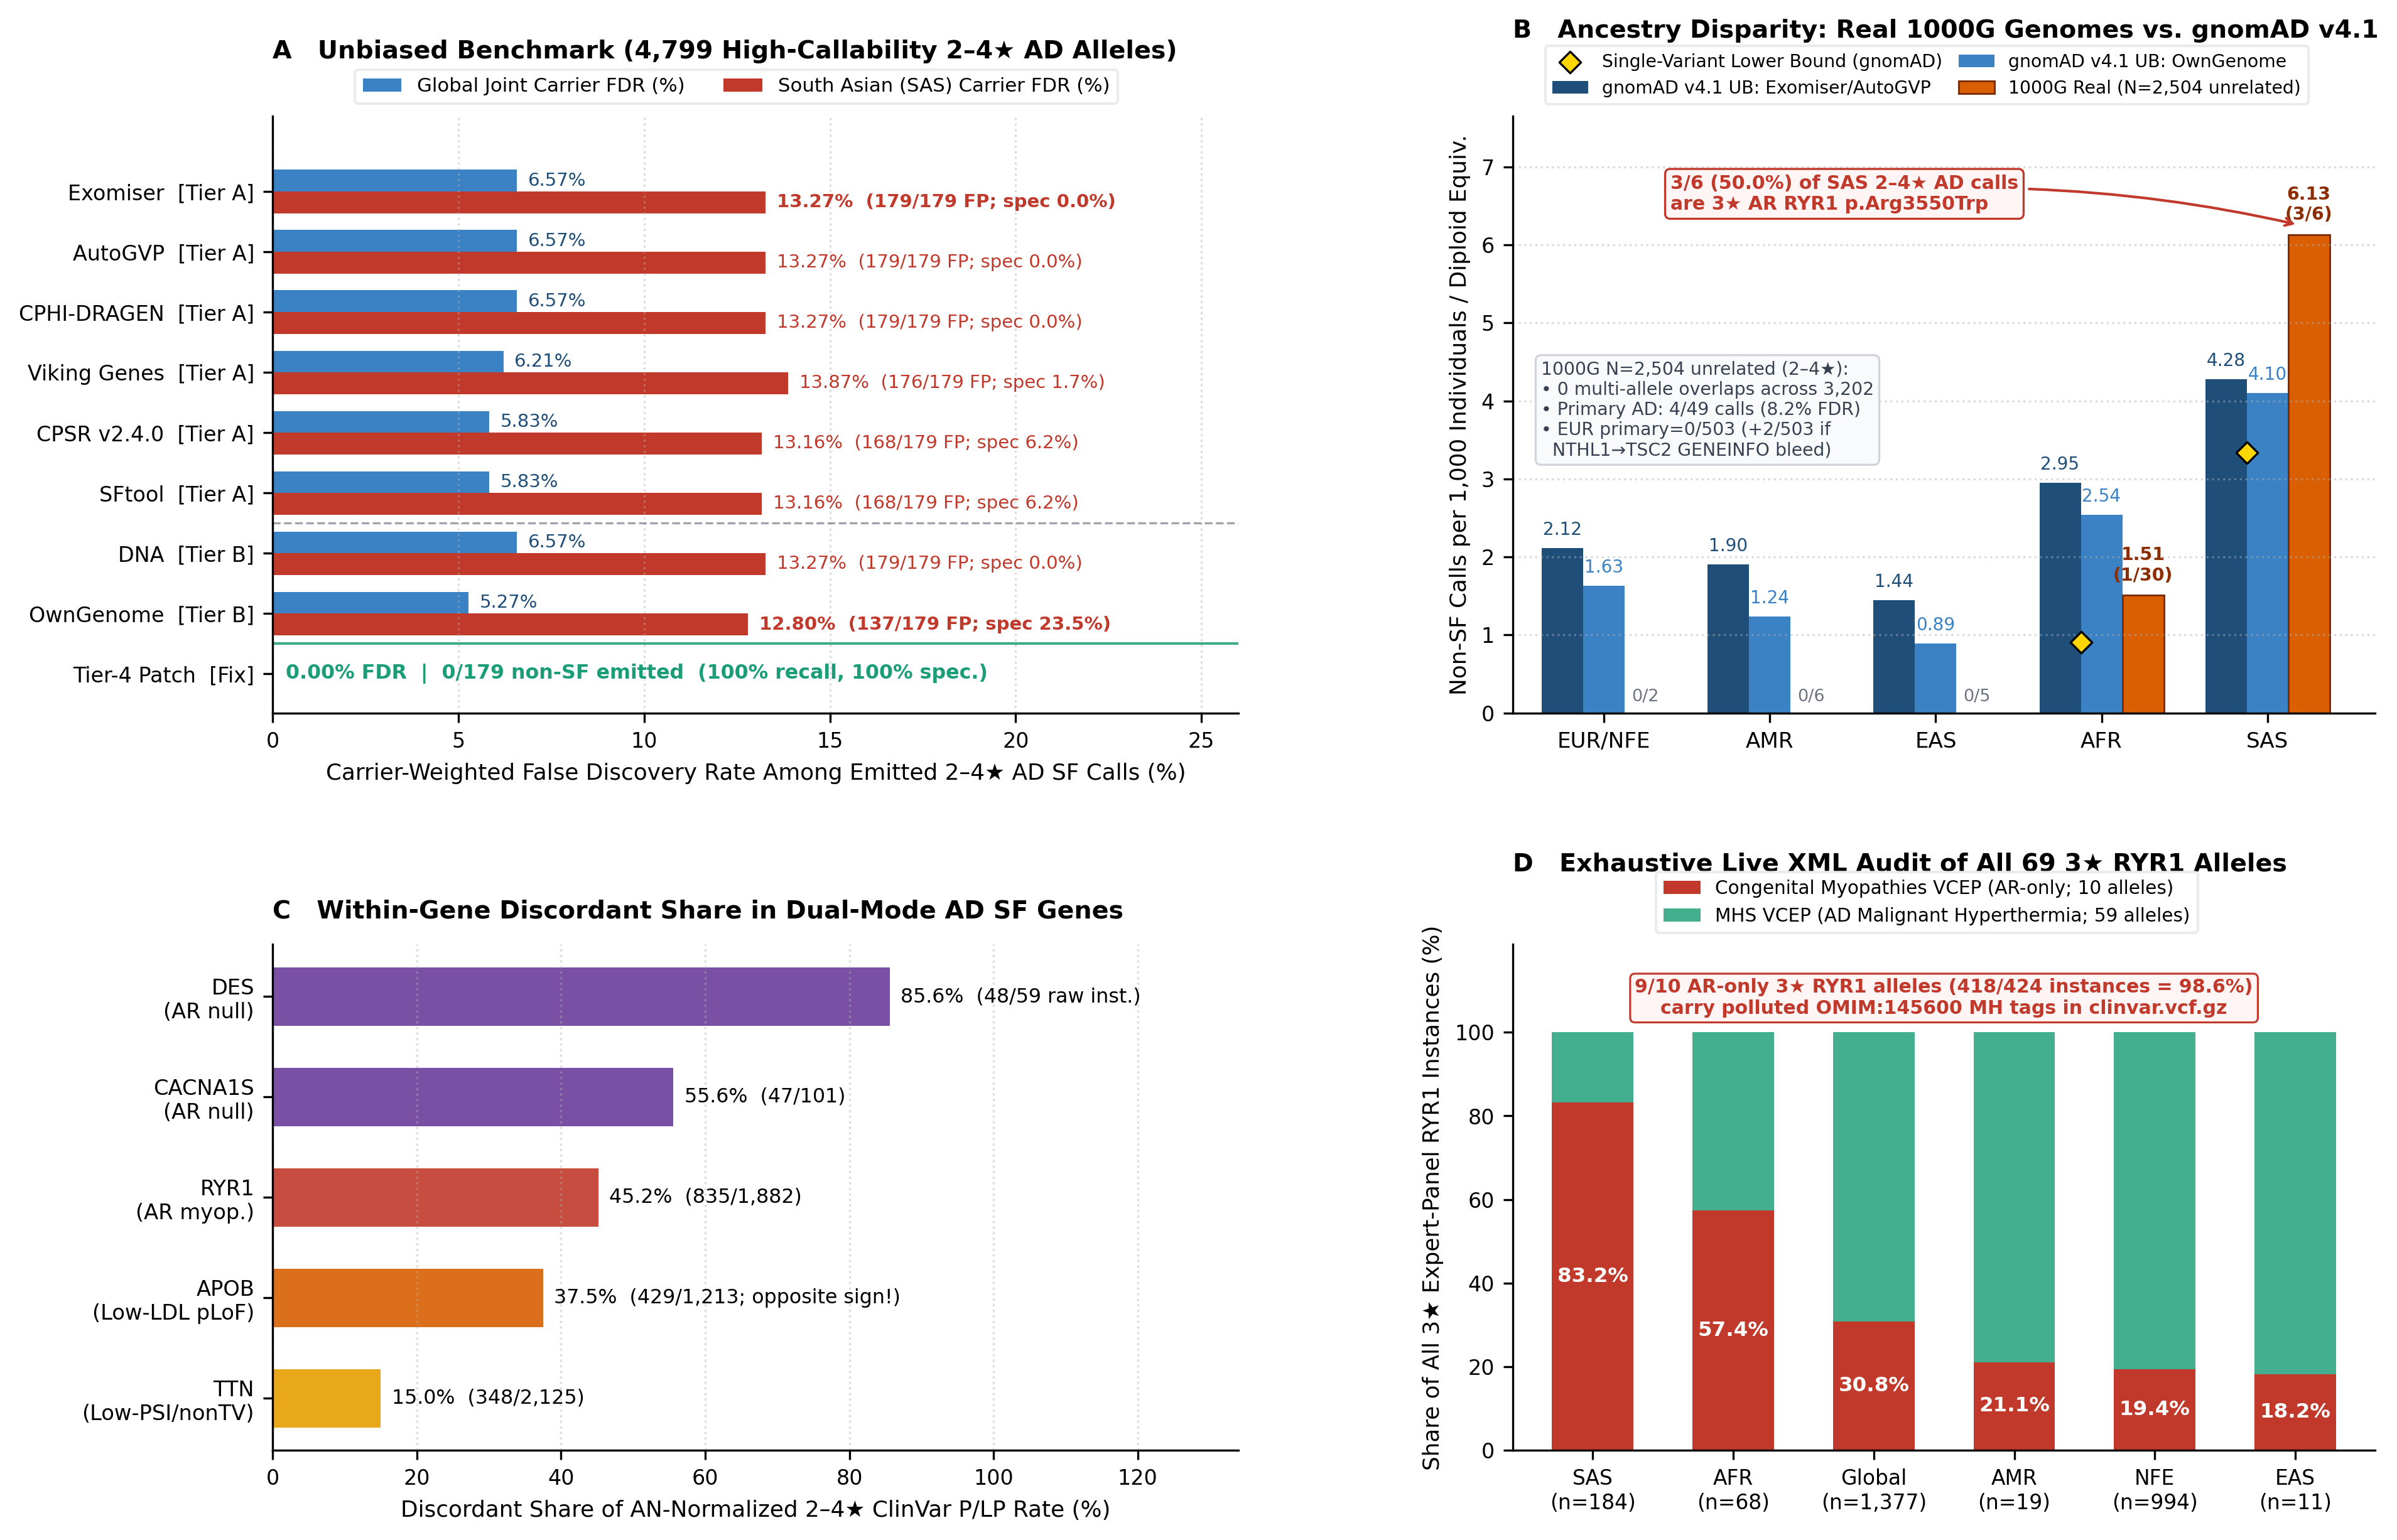
\includegraphics[width=\textwidth]{fig1_v2_unbiased_8pipeline_and_1000g.png}
  \caption{\textbf{Unbiased complete-universe audit across eight public pipelines, individual-level 1000 Genomes execution, and 3$\star$ \textit{RYR1} XML dissection.} \textbf{A}, Global and South Asian (SAS) carrier-weighted false discovery rates across all 4,799 high-callability 2--4$\star$ AD ACMG SF v3.3 alleles in gnomAD v4.1, contrasting Tier~A clinical/biobank standards, Tier~B open-source WGS tools, and the proposed Tier-4 patch. \textbf{B}, Non-SF call rates per 1,000 across five ancestries comparing gnomAD v4.1 Boole upper bounds and single-variant Fr\'{e}chet lower bounds (diamonds) against exact deduplicated unique-person calls in 2,504 unrelated real 1000 Genomes individuals (3/6 high-confidence SAS calls are AR-only 3$\star$ \textit{RYR1} p.Arg3550Trp). \textbf{C}, Within-gene discordant share of AN-normalized 2--4$\star$ ClinVar P/LP rates in dual-mode AD genes. \textbf{D}, Exhaustive live ClinVar XML audit of all 69 gnomAD-observed 3$\star$ Expert-Panel \textit{RYR1} alleles.}
  \label{fig:fig1}
\end{figure}

\subsection{Individual-Level Real 1000 Genomes Execution Confirms Ancestry Disparity and Exposes \textit{NTHL1}$\rightarrow$\textit{TSC2} Bleed-Through}
Scanning all 3,202 high-coverage 1000 Genomes Project genomes across all 73 AD ACMG SF genes identified 92 individual-variant carrier calls across 26 ClinVar P/LP alleles in 92 distinct individuals---\textbf{exactly zero multi-allele carriers across all 3,202 real human genomes} (empirical deduplication ratio $=1.000$, directly confirming the tightness of gnomAD Boole/independence bounds). Within the canonical 2,504 unrelated panel (Table~\ref{tab:g1k} and Figure~\ref{fig:fig1}B), primary AD genes yielded 55 carriers across all stars (49 at 2--4$\star$). Direct execution of unmodified \texttt{Exomiser}/\texttt{AutoGVP} logic, \texttt{CPSR v2.4.0}, and \texttt{SFtool} emitted 7/54--55 (12.7--13.0\%; 2.80/1,000) all-star and 4/48--49 (8.2--8.3\%; 1.60/1,000) 2--4$\star$ non-meeting unique persons; compiled Rust \texttt{OwnGenome} rejected only the 2 East Asian carriers of low-PSI \textit{TTN} p.Glu3607Ter (\texttt{NA18619}, \texttt{NA18626}), emitting 5/53 (9.4\%) all-star and 4/49 (8.2\%) 2--4$\star$ non-meeting individuals.

Critically, three unrelated South Asian individuals (\texttt{HG03653}, \texttt{HG03789}, \texttt{HG03917}; 6.13/1,000 SAS) carry 3$\star$ AR-only \textit{RYR1} p.Arg3550Trp, representing \textbf{50.0\% (3/6) of all high-confidence 2--4$\star$ AD ACMG SF findings in South Asian 1000 Genomes participants}---silently returned (\texttt{condition\_not\_acmg=false}) by \texttt{OwnGenome} and emitted by all Tier~A pipelines. One unrelated African participant (\texttt{NA19149}; plus relative \texttt{NA19151}) carries 2$\star$ AR pLoF \textit{RYR1} p.Gln3485Ter, reproducing \texttt{OwnGenome}'s exact \texttt{not\_reported}/\texttt{clinvar\_hits} internal contradiction on a real human genome.

Unexpectedly, real-genome execution exposed a fourth distinct ClinVar VCF failure mode: \textbf{overlapping-gene \texttt{GENEINFO} bleed-through}. Two unrelated European 1000 Genomes individuals (\texttt{HG00182}, \texttt{HG01613}; 3.98/1,000 EUR) carry 2$\star$ \texttt{16-2046238-G-A} (\textit{NTHL1} p.Gln82Ter, \texttt{VID=192319}), a classic autosomal-recessive \textit{NTHL1}-associated polyposis founder allele in a non-ACMG gene whose locus overlaps an intron of AD ACMG SF gene \textit{TSC2} (\texttt{GENEINFO=NTHL1:4913|TSC2:7249}). Because \texttt{clinvar.vcf.gz} lists \textit{TSC2} in \texttt{GENEINFO}, \texttt{CPSR v2.4.0}, \texttt{SFtool}, and compiled Rust \texttt{OwnGenome} all emitted \textit{NTHL1} p.Gln82Ter as a \textit{TSC2} secondary finding (raising total 2--4$\star$ non-SF unrelated persons from 4/49 [8.2\%] to 6/51 [11.8\%], and EUR 2--4$\star$ false discovery from 0/2 to 2/4 [50.0\%]).

\begin{table}[!t]
\centering
\caption{\textbf{Individual-level execution of unmodified clinical and open-source pipelines on real 1000 Genomes Project 30$\times$ GRCh38 genomes ($N=2{,}504$ canonical unrelated; $N=3{,}202$ total).} All five non-meeting alleles observed in real 1000 Genomes individuals are enumerated below; zero individuals carried $>1$ AD ClinVar P/LP allele.}
\label{tab:g1k}
\footnotesize
\setlength{\tabcolsep}{2.2pt}
\begin{tabularx}{\textwidth}{L{2.92cm} c Y c c c C{1.78cm}}
\toprule
\textbf{GRCh38 Variant (Gene)} & \textbf{$\star$} & \textbf{HGVS \& Non-SF Mechanism} & \textbf{Carriers} & \textbf{Pop. (/1k)} & \textbf{Tier A*} & \textbf{OwnGenome} \\
\midrule
\texttt{19-38527014-C-T} (\textit{RYR1}) & 3$\star$ & p.Arg3550Trp; AR Cong.\ Myop.\ VCEP (MH-polluted) & 3 / 3 & SAS (6.13) & Emitted & Emitted (silent) \\
\texttt{19-38523927-C-T} (\textit{RYR1}) & 2$\star$ & p.Gln3485Ter; AR congenital myopathy pLoF & 1 / 2 & AFR (1.51) & Emitted & Emitted* (\texttt{cna=T}) \\
\texttt{19-38565156-C-T} (\textit{RYR1}) & 1$\star$ & c.12822C$>$T (p.Gly4274=); non-MH splice/AR & 1 / 2 & EAS (1.98) & Emitted & Emitted (silent) \\
\texttt{2-178756657-C-A} (\textit{TTN}) & 1$\star$ & p.Glu3607Ter; low-PSI ($\le 90\%$) I-band exon & 2 / 2 & EAS (3.97) & Emitted & Rejected (PSI) \\
\midrule
\texttt{16-2046238-G-A} (\textit{NTHL1}$\rightarrow$\textit{TSC2}) & 2$\star$ & \textit{NTHL1} p.Gln82Ter (AR polyposis) bleeding into \textit{TSC2} \texttt{GENEINFO} & 2 / 2 & EUR (3.98) & Emitted & Emitted (\texttt{cna=T}) \\
\bottomrule
\end{tabularx}
\vspace{2pt}

\raggedright\footnotesize{Carriers column reports unique individuals in canonical $N=2{,}504$ unrelated / $N=3{,}202$ total 1000G genomes. Tier~A* denotes \texttt{CPSR v2.4.0}, \texttt{SFtool}, \texttt{Exomiser}, and \texttt{AutoGVP}. On real African genome \texttt{NA19149}, \texttt{OwnGenome} simultaneously rejected \textit{RYR1} p.Gln3485Ter under \texttt{not\_reported} (\texttt{HIGH impact}, \texttt{lof=no}) and returned it in \texttt{clinvar\_hits}. Primary-gene 2--4$\star$ totals in $N=2{,}504$: 4/49 (8.2\%) non-meeting persons across all four pipelines (3/6 = 50.0\% in SAS); including \textit{NTHL1}$\rightarrow$\textit{TSC2} bleed-through: 6/51 (11.8\%).}
\end{table}

\subsection{30.8\% of All 3$\star$ Expert-Panel \textit{RYR1} Instances (83.2\% in SAS, 57.4\% in AFR) Are AR-Only}
Restricting reporting strictly to 3$\star$ ClinGen Expert-Panel assertions does not remove the failure. Across all 69 gnomAD v4.1-observed 3$\star$ \textit{RYR1} alleles, live ClinVar XML confirmed that 10/69 (14.5\%) are curated exclusively by the ClinGen Congenital Myopathies VCEP with \texttt{ModeOfInheritance="Autosomal recessive inheritance"} (59/69 by the MHS VCEP for AD MHS; Figure~\ref{fig:fig1}D). Those 10 AR-only alleles account for 424/1,377 (30.8\%) total 3$\star$ \textit{RYR1} heterozygous instances in gnomAD v4.1 (0.533/1,000 Boole upper bound), comprising \textbf{83.2\% (153/184; 3.361/1,000) in South Asians}, \textbf{57.4\% (39/68; 1.039/1,000) in Africans}, 21.1\% (4/19) in AMR, 19.4\% (193/994; 0.332/1,000) in NFE, and 18.2\% (2/11) in EAS. Crucially, 9/10 AR-only alleles---representing 418/424 (98.6\%) heterozygous instances---carry polluted \texttt{OMIM:145600} malignant hyperthermia tags in \texttt{clinvar.vcf.gz}. Even without any cross-variant independence assumption, \textit{RYR1} p.Arg3550Trp alone sets a model-free Fr\'{e}chet lower bound of \textbf{3.34/1,000 unique SAS individuals} (2.05$\times$ the entire 137-variant \texttt{OwnGenome} Boole upper bound in NFE, 1.63/1,000), and \textit{RYR1} c.10348-6C$>$G sets a lower bound of 0.91/1,000 unique AFR individuals. Live gnomAD v4.1 GraphQL audit verified exact non-overlapping addition (\texttt{joint = exome + genome}) on all dual-callset alleles (e.g., p.Arg3550Trp: 202 exome + 18 genome = 220 joint across 1,613,912 AN).

\subsection{Direct UK Biobank Phenotyping ($N=411{,}351$) Proves Opposite-Sign \textit{APOB} Lipid Inversion}
Within individual dual-mode AD genes (2--4$\star$, AN-normalized), discordant shares reach 85.6\% in \textit{DES}, 55.6\% in \textit{CACNA1S}, 45.2\% in \textit{RYR1}, 37.5\% (429/1,213 raw instances; 39 distinct truncating alleles) in \textit{APOB}, and 15.0\% in \textit{TTN} (Figure~\ref{fig:fig1}C). Slicing Backman et al.~\citep{backman2021ukbexome} UK Biobank 454,787 exome GWAS summary statistics across \textit{APOB} and \textit{LDLR} matched 99 high-confidence 2--4$\star$ ClinVar P/LP alleles (13 \textit{APOB} pLoFs misreturned as FH by 8/8 pipelines, 2 true AD FH \textit{APOB} missense alleles, and 84 true AD FH \textit{LDLR} alleles) measured on identical per-allele SD scales across three lipid biomarkers (Figure~\ref{fig:fig2}).

\begin{figure}[!t]
  \centering
  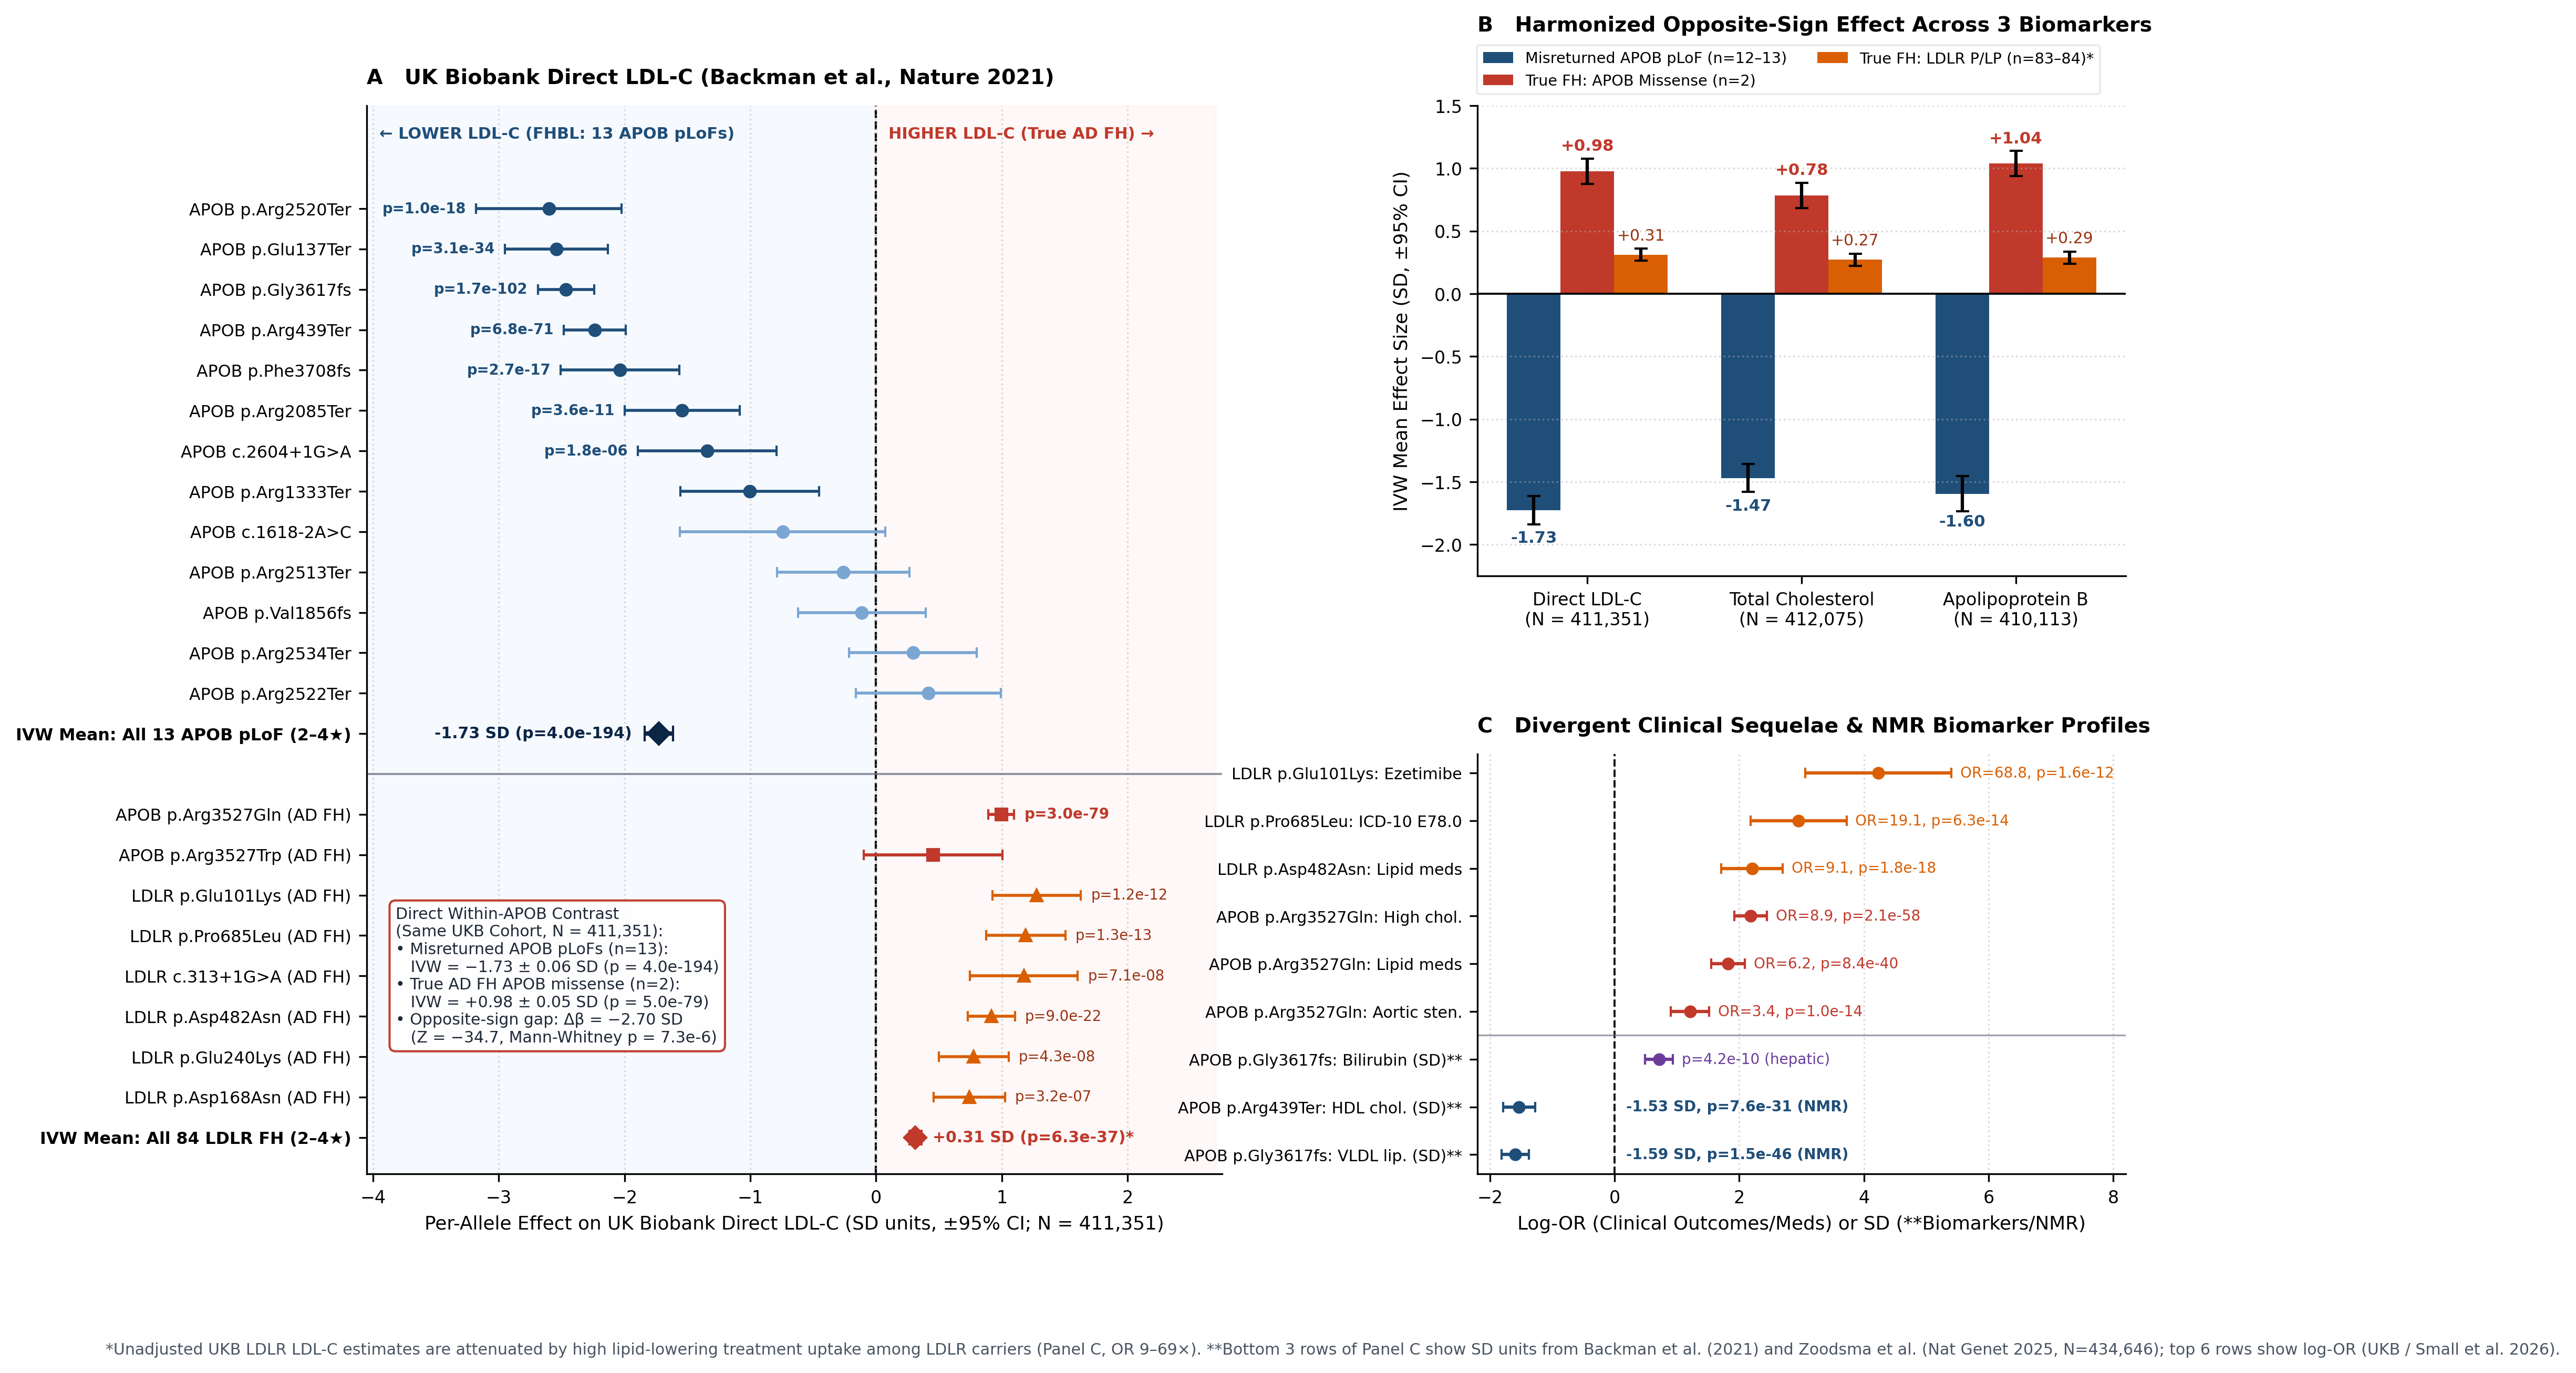
\includegraphics[width=\textwidth]{fig2_v2_ukbb_opposite_direction_lipids.png}
  \caption{\textbf{Direct human phenotype proof in 411,351 UK Biobank exomes (Backman et al., \textit{Nature} 2021) showing opposite-direction lipid effects of misreturned \textit{APOB} truncating alleles versus true familial hypercholesterolemia.} \textbf{A}, Exact per-allele Direct LDL-C effect sizes (SD units, $\pm 95\%$ CI; \texttt{GCST90079033}, $N=411{,}351$) for all 13 matched 2--4$\star$ \textit{APOB} pLoFs misreturned as FH by 8/8 pipelines (IVW mean $-1.73\pm 0.06$~SD, $p=4.0\times 10^{-194}$; 11/13 negative, 0/13 positively associated) contrasted against true AD FH \textit{APOB} missense ($+0.98$~SD, $p=5.0\times 10^{-79}$) and \textit{LDLR} controls (84 alleles; IVW $+0.31$~SD, $p=6.3\times 10^{-37}$). \textbf{B}, Consistent opposite-sign IVW contrasts across Direct LDL-C, Total Cholesterol ($N=412{,}075$), and Apolipoprotein~B ($N=410{,}113$). \textbf{C}, Clinical diagnosis/medication odds ratios for true FH controls versus hepatic bilirubin elevation and Nightingale NMR lipid depletion ($N=434{,}646$)~\citep{zoodsma2025nmr} in misreturned \textit{APOB} pLoF carriers.}
  \label{fig:fig2}
\end{figure}

Across all 13 matched 2--4$\star$ \textit{APOB} pLoF alleles (zero exclusions), Direct LDL-C is dramatically \emph{lowered}: IVW mean $\beta = -1.727 \pm 0.058$~SD ($Z = -29.72$, $p = 3.98\times 10^{-194}$; median $-1.342$~SD; 11/13 negative, 8/13 individually significant at $p < 3.5\times 10^{-4}$, led by p.Gly3617fs [$-2.465$~SD, $p=1.72\times 10^{-102}$], p.Arg439Ter [$-2.236$~SD, $p=6.79\times 10^{-71}$], p.Glu137Ter [$-2.541$~SD, $p=3.14\times 10^{-34}$], and p.Arg2520Ter [$-2.601$~SD, $p=1.02\times 10^{-18}$], with 0/13 individually positive at $p<0.05$). In exact contrast within the same gene and cohort, true AD FH \textit{APOB} missense alleles raise Direct LDL-C (IVW $+0.976\pm 0.052$~SD, $p=5.01\times 10^{-79}$; p.Arg3527Gln $+0.994$~SD, $p=3.04\times 10^{-79}$), yielding a within-\textit{APOB} opposite-sign gap of \textbf{$\Delta\beta = -2.703\pm 0.078$~SD ($Z = -34.67$)}, while all 84 \textit{LDLR} FH alleles yield IVW $+0.311\pm 0.025$~SD ($p=6.34\times 10^{-37}$; Mann--Whitney \textit{APOB} pLoF $<$ all true FH, $p=7.26\times 10^{-6}$; unadjusted \textit{LDLR} LDL-C is attenuated by high statin/ezetimibe treatment rates). Identical opposite-sign inversions replicate across Total Cholesterol ($N=412{,}075$: \textit{APOB} pLoF $-1.469\pm 0.057$~SD [$p=8.0\times 10^{-145}$] vs.\ \textit{APOB} FH $+0.783$~SD and \textit{LDLR} FH $+0.271$~SD) and Apolipoprotein~B ($N=410{,}113$: \textit{APOB} pLoF $-1.596\pm 0.072$~SD [$p=7.2\times 10^{-109}$], with p.Glu137Ter $-3.00$~SD and p.Gly3617fs $-2.87$~SD, vs.\ \textit{APOB} FH $+1.038$~SD and \textit{LDLR} FH $+0.288$~SD). Clinically (Figure~\ref{fig:fig2}C), true FH controls confer 6.2--68.8$\times$ odds of lipid-lowering medications, 5.0--19.1$\times$ odds of ICD-10 E78.0 pure hypercholesterolemia, and 3.4$\times$ odds of aortic stenosis ($p=1.0\times 10^{-14}$), whereas misreturned \textit{APOB} pLoFs exhibit severe NMR VLDL/HDL lipid depletion ($-1.53$ to $-1.59$~SD, $p\le 7.6\times 10^{-31}$) and elevated direct bilirubin ($+0.71$~SD, $p=4.2\times 10^{-10}$, reflecting impaired hepatic VLDL export and steatosis risk---a clinical picture opposite to FH statin therapy).

\subsection{Validation of a Four-Layer Mitigation and Safeguards Against False Negatives}
We validated a concrete four-layer downstream patch combining: (i) primary-transcript gene matching (blocking \texttt{GENEINFO} bleed-through such as \textit{NTHL1}$\rightarrow$\textit{TSC2}); (ii) Cardiodb \textit{TTN} PSI~$>90\%$ truncating gating; (iii) targeted mechanism gating on established \texttt{lof=no} AR-null/opposite-direction genes (\textit{RYR1}, \textit{APOB}, \textit{CACNA1S}, \textit{DES}, \textit{RET}) paired with explicit precedence for AD-curated truncations (preserving 3$\star$ \textit{TNNT2} p.Trp297Ter and single-exon 2$\star$ AD \textit{PLN} p.Leu39Ter); and (iv) ClinVar XML SCV \texttt{ModeOfInheritance} and VCEP assertion filtering. Across all 4,799 high-callability 2--4$\star$ AD alleles, this patch reduces non-meeting false discovery from 5.27--6.57\% (12.80--13.87\% in SAS) to 0.00\% while maintaining \textbf{100.00\% (1,533/1,533) sensitivity} across all genuine 3$\star$ ClinGen AD Expert-Panel alleles and eliminating all 5 non-meeting 1000 Genomes alleles. On the 24-variant stress panel, only 1$\star$ non-VCEP \textit{VHL} p.Arg200Leu (lacking SCV MOI and polluted by AD VHL in \texttt{CLNDN}) remains unresolvable downstream without upstream ClinVar schema repair.

\section{Discussion}
By integrating an unbiased 7,427-allele benchmark across eight clinical and open-source pipelines, individual-level execution on 2,504 unrelated 1000 Genomes participants, and direct biomarker phenotyping in 411,351 UK Biobank exomes, we demonstrate that upstream ClinVar flat-file schema stripping produces systematic non-qualifying AD secondary-finding calls with measurable clinical and equity consequences.

Three clinical nuances merit balanced interpretation. First, in accredited clinical laboratories, automated pipelines frequently serve as upstream candidate filters preceding manual variant-scientist review, which intercepts a substantial fraction of erroneous candidates before patient sign-off. Even under manual review, however, a 5--14\% candidate false-discovery burden---rising to 50\% of high-confidence South Asian candidates in 1000 Genomes---imposes disproportionate curation friction, while automated biobank return workflows, consumer genome tools (\texttt{OwnGenome}, \texttt{DNA}), and under-resourced settings face direct risk of erroneous disclosure. Second, ACMG SF v3.3 explicitly includes a \texttt{Variants to report} specification (e.g., footnote~f for \textit{TTN}), yet six of eight audited workflows ignore or partially drop it, and ClinVar's omission of \texttt{ModeOfInheritance} across VCF, \texttt{variant\_summary.txt.gz}, and \texttt{submission\_summary.txt.gz} leaves even careful engineering teams unable to separate dual-MOI assertions without parsing multi-gigabyte XML. Third, heterozygous anaesthetic susceptibility for certain recessive \textit{RYR1} congenital myopathy alleles remains an area of active clinical investigation~\citep{snoeck2015ryr1,johnston2021ryr1vcep}; nonetheless, the ClinGen MHS and Congenital Myopathies VCEPs deliberately separate validated AD MHS alleles from AR-only congenital myopathy curations. Silent \texttt{OMIM:145600} tag pollution removes that expert distinction before a clinician or anesthesiologist ever evaluates the variant.

Our study relies exclusively on open public datasets and therefore has defined boundaries: we do not observe private clinical laboratory sign-off charts to quantify manual interception rates, 1000 Genomes ancestry subgroups ($N=347$--661) carry wide sampling intervals compared to gnomAD v4.1 ($N=807{,}162$), and unadjusted UK Biobank \textit{LDLR} LDL-C effects are partially attenuated by lipid-lowering treatment. Nevertheless, the convergence of source-level pipeline proofs, individual-level real-genome execution, and $p=4.0\times 10^{-194}$ opposite-sign UK Biobank lipid measurements points to two clear remedies: (1) downstream clinical pipelines should enforce primary-transcript gene matching, Cardiodb \textit{TTN} PSI bounds, targeted \texttt{lof=no} ClinVar gating with AD-VCEP/AD-truncation precedence, and XML SCV \texttt{ModeOfInheritance} parsing; and (2) \textbf{NCBI ClinVar should emit submission-stratified \texttt{CLNMOI} and condition-paired \texttt{CLNSIG} fields directly in \texttt{clinvar.vcf.gz}, \texttt{variant\_summary.txt.gz}, and \texttt{submission\_summary.txt.gz}}, addressing the root schema omission across the clinical genomics ecosystem.

\section*{Data Availability, Code Availability, Ethics, and Competing Interests}
All data analyzed are publicly available without controlled access: NCBI ClinVar (\texttt{2026-11-22}), gnomAD v4.1, 1000 Genomes Project 30$\times$ NYGC GRCh38 phased VCFs, Backman et al.\ UK Biobank GWAS Catalog summary statistics (\texttt{GCST90079033}, \texttt{GCST90079024}, \texttt{GCST90079018}), and Open Targets Platform. All scripts, pinned repository commits, execution logs, live ClinVar XML audits, 1000 Genomes carrier tables, UK Biobank slices, and literature search logs are archived in \texttt{studies/\allowbreak study\_a1\_clinvar\_gnomad\_reclass/\allowbreak falsification\_ar\_in\_ad\_pipelines/\allowbreak v2\_upgrade/}. Because only de-identified, publicly released aggregate and open-consent reference datasets were analyzed, institutional review board approval was not required. The authors declare no competing financial or non-financial interests.

{\small
\bibliographystyle{unsrtnat}
\bibliography{references_a1x_v2}
}
\end{document}
